\documentclass[times, utf8, zavrsni]{fer}
\usepackage{booktabs}
\usepackage{listings}
\usepackage{color}

\definecolor{dkgreen}{rgb}{0,0.6,0}
\definecolor{gray}{rgb}{0.5,0.5,0.5}
\definecolor{mauve}{rgb}{0.58,0,0.82}

\lstset{frame=tb,
  language=Java,
  aboveskip=3mm,
  belowskip=3mm,
  showstringspaces=false,
  columns=flexible,
  basicstyle={\small\ttfamily},
  numbers=none,
  numberstyle=\tiny\color{gray},
  keywordstyle=\color{blue},
  commentstyle=\color{dkgreen},
  stringstyle=\color{mauve},
  breaklines=true,
  breakatwhitespace=true,
  tabsize=3
}

\begin{document}

% TODO: Navedite broj rada.
\thesisnumber{012}

% TODO: Navedite naslov rada.
\title{Višezadaćni rad, sinkronizacijski mehanizmi i upravljanje spremnikom u Android okruženju}

% TODO: Navedite vaše ime i prezime.
\author{Hrvoje Kozak}

\maketitle

% Ispis stranice s napomenom o umetanju izvornika rada. Uklonite naredbu \izvornik ako želite izbaciti tu stranicu.
% \izvornik

% Dodavanje zahvale ili prazne stranice. Ako ne želite dodati zahvalu, naredbu ostavite radi prazne stranice.
\zahvala{}

\tableofcontents

\chapter{Uvod}
Uvod rada. Nakon uvoda dolaze poglavlja u kojima se obrađuje tema.

\chapter{Upravljanje memorijom}
\section{Kako operacijski sustav Android upravlja memorijom}
\paragraph{}
Android ne nudi prostor za zamjenu \textit{(engl. swap)} za memoriju, već u tu svrhu koristi straničenje \textit{(engl. paginig)} i mapiranje memorije \textit{(engl. memory-mapping)}.\\

\textbf{Straničenje} \textit{(engl. paging)} je način na koji se spremaju i dohvaćaju podaci s vanjskog spremnika u glavnu memoriju. Operacijski sustav će te podatke dohvaćati u blokovima iste veličine i jedan takav blok zove se stranica. Ova tehnika isto tako važan je dio u implementaciji virtualne memorije, gdje se onda korištenjem vanjskog spremnika omogućava programima da prerastu dostupnu fizičku memoriju.\\

\textbf{Datoteka mapirane memorije} \textit{(engl. Memory-mapped file)} je segment virtualne memorije kojem se dodjeljuje direktna bajt po bajt korelacija s nekom datotekom ili sličnim resursom. Tipično je to datoteka koja se nalazi fizički na disku, ali može biti i uređaj ili objekt dijeljene memorije. Nakon povezanog mapiranja između datoteke i virtualne memorije aplikaciji se omogućava da tretira mapirani dio kao primarnu memoriju.\\

To bi značilo da kada god se koristi memorija, bilo alociranjem novih objekata ili korištenjem mapiranih stranica, ona ostaje unutar radne memorije i ne sprema se na vanjsku stranicu. Stoga, jedini način da se kompletno otpusti memorija iz aplikacije je otpuštanje referenci na objekte koji su trenutno u memoriji, nakon čega će ta memorija biti počišćena u procesu prikupljanja otpada. Postoji jedna iznimka, datoteke mapirane u sustav koje nisu mijenjane (npr. Izvorni kod) mogu se izvaditi u stranicu izvan radne memorije ako sustav trenutno želi koristiti tu memoriju u druge svrhe.

\subsection{Dijeljenje memorije}
\paragraph{}
Da bi uspjeli ubaciti sve u memoriju što nam je potrebno, procesi su primorani dijeliti stranice radnog spremnika. Samo dijeljenje stranica između procesa događa se na sljedeći način:

\begin{enumerate}
\item
Svaki proces aplikacije se račva \textit{(engl. fork)} od glavnog postojećeg procesa zvanog Zigota. Proces Zigote započinje svoj život odmah nakon što se uređaj pokrene \textit{(engl. boot)} i učita izvorni kod radnog okruženja \textit{(engl. framework)} i resurse. Prilikom pokretanja novog procesa aplikacije, sustav račva Zigotu, te učita i pokrene izvorni kod aplikacije u novom procesu. Time se dobiva efekt da većina RAM stranica alociranih za radno okruženje i resurse bude dijeljena na svim živim procesima.

\item
Većina statičnih podataka je mapirano u proces. Na taj su način ti podaci automatski podijeljeni s drugim procesima i mogu se zapisati u stranice ako je potrebno.

\item
Na puno mjesta, Android dijeli isti dinamički radni spremnik na više procesa pomoću eksplicitno alocirane regije djeljene memorije (korištenjem \textit{ashmem} ili \textit{gralloc} naredbi).
\end{enumerate}

\subsection{Alociranje i oslobađanje memorije aplikacije}
\paragraph{}
Za svaki proces, hrpa virtualne mašine Dalvik limitirana je na samo jednu virtualnu memoriju. To određuje logičku veličinu hrpe, koja raste po potrebi i koja ne mora nužno biti jednaka količini fizičke memorije koju hrpa koristi. Dalvik hrpa ne sažima logičku veličinu hrpe, što znači da ne radi nikakvu fragmentaciju. Jedino u slučaju pojavljivanja neiskorištenog prostora na kraju hrpe operacijski sustav može sažeti logičku veličinu hrpe.\\

Što se tiče fizičke memorije koju koristi hrpa, ona se može smanjiti. Nakon prikupljanja smeća, Dalvik prolazi kroz hrpu i nalazi nekorištene stranice koje onda vraća nazad \textit{kernelu} (naredbom \textit{madvise}). Treba primijetiti da ako imamo alokacije uparene s oslobađanjem, kod velikih komada memorije može se očekivati da će sva memorija biti vraćena. S druge strane manje efektivan je slučaj kada se promatraju manje alokacije jer stranica korištena za manje alokacije može biti dijeljena s nečime što se još nije oslobodilo.

\subsection{Ograničavanje memorije aplikacije}
\paragraph{}
Da bi održao funkcionalno više-dretveno (engl. multi-threading) okruženje, Android svakoj aplikaciji postavlja limit na njezinu veličinu hrpe. Taj limit varira i ovisi o samom uređaju, a baziran je na ukupnoj količini radne memorije na uređaju. U slučaju da aplikacija pokuša alocirati memoriju u trenutku kada je već dosegla svoj limit, dobiti će \textit{OutOfMemoryError}.\\

Provjera slobodnog prostora na hrpi može se pozvati \textit{getMemoryClass()} metoda. Ona će vratiti \textit{integer} koji pokazuje količinu slobodnih megabajta na hrpi za našu aplikaciju.

\subsection{Mijenjanje aplikacije od strane korisnika}
\paragraph{}
Kao što smo rekli Android nema prostor za zamjenu. Iz tog razloga, kada se korisnik prebacuje iz jedne aplikacije u drugu, Android sprema trenutno nevidljive procese u LRU \textit{(engl. Least Recently Used)} priručnu memoriju \textit{(engl. cache)}. Znači nakon što korisnik napusti aplikaciju, proces se ne ubija nego se sprema u priručnu memoriju sa svrhom ponovnog korištenja i bržih promjena aplikacija na uređaju.\\

Naravno dok se aplikacija ne koristi, pošto je spremljena u priručnoj memoriji, ona još uvijek koristi memorijski prostor. Ako sustavu nedostaje memorije, može odlučiti ubiti jednu od aplikacija u priručnoj memoriji. Odluku će donijeti na temelju procjene koja je aplikacija najmanje korištena u posljednje vrijeme, ili  koja od njih agresivno konzumira memoriju.

\pagebreak
\section{Upravljanje memorijom u Android aplikacijama}
\paragraph{}
Pri izradi Android aplikacija treba biti svijestan ograničenja memorije tokom svih faza razvoja, pa čak i prilikom izrade dizajna aplikacije neposredno prije samog početka razvoja. Takvim pristupom izbjegava se jako puno grešaka \textit{(engl. bug)} i curenja memorije \textit{(engl. memory leak)}, te se štedi vrijeme samog razvoja aplikacije. Postoje razne tehnike i dobre prakse vezane uz dizajn i pisanje koda koje povlače bolju kvalitetu same aplikacije i manje problema s memorijom, a u nastavku će se proći kroz one najbitnije.

\subsection{Pažljivo baratanje servisima}
\paragraph{}
Pri korištenju nekog servisa za odrađivanje posla u pozadini, mora se jako paziti da  ne ostane pokrenut u trenucima kada ne obavlja aktivno niti jedan posao. Isto tako ne smije se dogoditi da servis procuri, što se događa kada ga se zaboravi zaustaviti nakon obavljenog posla. Takav propust smatra se jednom od najgorih grešaka kod upravljanja memorijom jer ne samo da će aplikacija lošije funkcionirati, nego će i korisnici primijetiti neočekivana ponašanja i pobrisati aplikaciju s uređaja.\\

Najbolji način za limitiranje životnog spektra servisa je korištenje \textit{IntentService} klase, koja će se sama počistiti odmah nakon što odradi stvar zbog koje je pozvana.

\subsection{Otpuštanje memorije}
\paragraph{}
U bilo kojem trenutku života aplikacije, ugrađeni poziv \textit{(engl. callback)} \textit{onTrimMemory()} obavještava kada sveukupna memorija uređaja postaje premala. Na taj ugrađeni poziv trebalo bi odgovoriti otpuštanjem memorije resursa koji se drže u aplikaciji, a odluka o tome koje i koliko resursa otpustiti donosi se s obzirom na zaprimljeni nivo memorije od strane \textit{onTrimMemory()}. Nivoi memorije su sljedeći:

\paragraph{•}
\verb|TRIM_MEMORY_UI_HIDDEN|\\
Ovo je jedna od najvažnijih zastavica i indicira da je korisničko sučelje \textit{(engl. User Interface, UI)} trenutno skriveno od korisnika (npr. kada se korisnik navigira u drugu aplikaciju). To je signal da se trebaju osloboditi svi resursi koje trenutno koristi UI i tako znatno povećati kapacitet operacijskog sustava za spremanje procesa u priručnu memoriju, što je u krajnjoj liniji direktno poboljšanje kvalitete korisničkog korištenja aplikacije \textit{(engl. User Experience, UX)}.

\paragraph{•}
\verb|TRIM_MEMORY_RUNNING_MODERATE|\\
Naša aplikacija nije direktno ugrožena, sustav javlja da je slab s memorijom i počinje aktivno ubijati procese u LRU priručnoj memoriji.

\paragraph{•}
\verb|TRIM_MEMORY_RUNNING_LOW|\\
Naša aplikacija nije direktno ugrožena, sustav javlja da je puno slabiji s memorijom i ovdje bi se trebali već poćeti oslobađati nekorišteni resursi u aplikaciji.

\paragraph{•}
\verb|TRIM_MEMORY_RUNNING_CRITICAL|\\
Naša aplikacija još uvijek živi, ali sustav je već ubio većinu procesa u LRU priručnoj memoriji. Ovdje se trebaju otpustiti svi resursi koji nisu krucijalni za nastavak rada aplikacije.\\

\noindent
Ukoliko je naš proces već u priručnoj memoriji možemo očekivati sljedeće zastavice:

\paragraph{•}
\verb|TRIM_MEMORY_BACKGROUND|\\
Sustav je slab s memorijom, a naš proces je negdje na početku LRU liste. Iako naš proces nema prevelik rizik da bude uništen ubrzo, ovo je signal da se LRU priručna memorija već počinje čistiti i ovdje bi trebali osloboditi sve resurse koje je kasnije lako povratiti.

\paragraph{•}
\verb|TRIM_MEMORY_MODERATE|\\
Sustav je slab s memorijom, a naš proces je negdje na sredini LRU liste i postoji dobra šansa da se naš proces uništi ako proces zatraži još dodatne memorije.

\paragraph{•}
\verb|TRIM_MEMORY_COMPLETE|\\
Sustav je slab s memorijom, a naš proces je prvi koji će biti uništen ako sustav u tom trenutku ne uspije osloboditi dovoljno memorije. Ovdje treba otpustiti apsolutno sve što nije krucijalno za nastavak rada aplikacije.\\

Ovaj \textit{onTrimMemory()} ugrađeni poziv je dodan tek u API verzije 14 tako da za starije verzije uređaja treba koristiti \textit{onLowMemory()} ugrađeni poziv koji se u principu ponaša isto kao i \verb|TRIM_MEMORY_COMPLETE| \textit{event}.

\subsection{Provjera dostupne memorije}
\paragraph{}
Kako je svaki android uređaj drukčiji i njegova količina radne memorije varira, isto tako mijenja se i limit veličine hrpe za svaku aplikaciju na uređaju. U slučaju da aplikacija pokuša alocirati memoriju u trenutku kada je već dosegla svoj limit, dobiti će \textit{OutOfMemoryError}, a pozivom na \textit{getMemoryClass()} dobit će se procjena dostupne memorije za aplikaciju u megabajtima.\\

U posebnim slučajevima može se zatražiti veća količina hrpe postavljanjem atributa \textit{largeHeap} na \textit{true} unutar \textit{manifest} \verb|<application>| taga. Tada se procjena dostupne memorije za tu veću hrpu dobiva pozivom \textit{getLargeMemoryClass()} metode.\\

Naravno to se nikako ne smije koristiti kao lako rješenje svaki puta kada se ostane bez memorije. Ovakav pristup namijenjen je malom broju aplikacija koje mogu opravdati potražnju za većom količinom memorije.

\subsection{Skaliranje bitmapa}
\paragraph{}
Prilikom učitavanja \textit{bitmap} datoteke, cilj je u memoriji držati samo rezoluciju koja nam treba za ekran trenutnog uređaja. Ako je originalna \textit{bitmap} datoteka prevelika, skalirat ćemo ju na željenu veličinu. Ovime se štedi jako puno memorije jer količina memorije za držanje \textit{bitmap} datoteke raste kvadratno s porastom veličine grafike (jer rastu X i Y osi).

\subsection{Optimizirani spremnici podataka}
\paragraph{}
Radno okruženje Android nam nudi strukture za spremanje podataka koje su optimizirane za Android OS, kao na primjer \textit{SparseArray, SparseBooleanArray i LongSparseArray}. Ako uzmemo za primjer implementaciju \textit{HashMap} strukture, ona može biti jako neugodna za memoriju jer prilikom svakog mapiranja stvara novi objekt. S druge strane \textit{SparseArray} klase su optimizirane tako da izbjegavaju potrebu automatske konverzije iz primitiva u klasu objekta \textit{(engl. autoboxing)}(npr. int u Integer) ključa, a ponekad i same vrijednosti.\\

Isto tako možemo iskoristiti i bazične \textit{Java} nizove kada to ima smisla.

\subsection{Dodatni troškovi memorije}
\paragraph{}
U izradi aplikacije jedna od najbitnijih stvari koje trebamo pripaziti je cijene i dodatni troškovi \textit{(engl. overhead)} jezika i radnog okruženja koje koristimo. Često se ljudi naviknu uzimati stvari zdravo za gotovo i rade greške koje na prvi pogled izgledaju nevino, dok ustvari troše veliku količinu memorije.

\paragraph{•}
Enumeracije \textit{(engl. Enumerations, Enum)} često zahtjevaju i do duplo više memorije od statičkih konstanta. Njih bi svakako trebali izbjegavati.

\paragraph{•}
Svaka klasa u \textit{Javi} koristi približno 500 bajta koda.

\paragraph{•}
Svaka instanca klase ima 12-16 bajta dodatnog troška u radnom spremniku.

\paragraph{•}
Stavljanje jednog unosa u \textit{HashMap}, zahtjeva alokaciju još jednog dodatnog objekta veličine 32 bajta.\\

Iako u prvu ruku ne izgleda kao prevelika štednja, kada se ovakve sitnice  skaliraju to jako brzo postaje veliki problem iz perspektive memorije.

\subsection{Apstrakcija koda}
\paragraph{}
Iako je apstrakcija koda dobra praksa u programiranju jer svojom fleksibilnošću olakšava održavanje aplikacije, ona dolazi s cijenom, a cijena je puno veća količina koda koji se treba izvesti, što povlači za sobom više radne memorije. Ako apstrakcije ne olakšavaju strukturu i fleksibilnost koda moraju se izbjegavati, jer će memorija biti jako zahvalna na tome.

\subsection{Mehanizam za serijalizaciju Protobuffs}
\paragraph{}
\textit{Protobuffs (Protocol buffers)} je mehanizam razvijen od strane \textit{Google-a} za serijalizaciju struktura podataka neovisni o jeziku i platformi. Nešto poput XML-a, međutim puno brži, manji i jednostavniji. Ako se koristi u kodu, na Android operacijskom sustavu uvijek bi se trebala uzeti nano verzija protobuffs mehanizma na klijentskoj strani koda. Time se značajno smanjuje korištenje memorije i veličina APK arhive, te se pritom ubrzava samo izvođenje programa.

\subsection{Ubrizgavanje zavisnosti}
\paragraph{}
Kada se koristi neko radno okruženje za ubrizgavanje zavisnosti (engl. dependency injection) kao \textit{Dagger} ili \textit{Guice}, iako olakšavaju samo kodiranje i testiranje aplikacije kontrolom dependency-a, moramo paziti na činjenicu da oni rade jako puno inicijalizacije procesa tijekom skeniranja našeg koda tražeći anotacije i time mapiraju u radnu memoriju značajnu količinu koda iako nam taj kod u memoriji i ne treba. Te stranice su mapirane u čistu memoriju kako bi ih Android mogao počistiti, no to će se dogoditi tek nakon što stranice odstoje u memoriji neko vrijeme nekorištene.

\subsection{Eksterne biblioteke}
\paragraph{}
Na eksterne biblioteke treba uvijek posebno paziti, pogotovo kada ih se koristi više u jednom projektu. Prvo se dolazi do problema kada biblioteka nije optimizirana za korištenje na mobilnim uređajima, u kojem će se slučaju morati preuzeti pisanje optimizacije i održavanje tog koda. S druge strane i onda kada su biblioteke navodno optimizirane za mobilne uređaje, tu imamo potencijalni problem kada više njih rade istu stvar na različite načine i javljaju se veliki dodatni troškovi memorije. Na primjer, ako koristimo dvije biblioteke s različitim implementacijama za \textit{logging, caching, analytics} i slično.

\subsection{Proguard}
\paragraph{}
Proguard je jako koristan alat koji smanjuje, optimizira i pomućuje (engl. obfuscates) kod. To radi tako da makne kod koji se ne koristi, te zamijeni imena varijabli, klasa i metoda sa semantički besmislenim imenima. 

\subsection{Poravnavanje finalne APK arhive}
\paragraph{}
Nakon što se potpiše produkcijska verzija aplikacije mora se i poravnati \textit{zipalign} alatom. U protivnom, aplikacija će trošiti znatno više radne memorije, jer se resursi neće moći automatski mapirati iz APK-a.

\begin{center}
\verb|zipalign [-f] <alignment> infile.apk outfile.apk|
\end{center}

Za \textit{alignment} parametar koristi se 4 bajta na android okruženju, a zastavica –f forsira prepisivanje rezultata preko postojeće \textit{outfile.apk} datoteke.

\subsection{Analiza korištenja radne memorije}
\paragraph{}
Da bi se dobio bolji uvid u funkcionalnost naše aplikacije, svaki stabilan build bilo bi dobro analizirati.
Prvi I najjednostavniji način je čitanje informacijskih poruka (engl. log) sakupljača smeća. Dok Dalvik svaki put printa poruke sakupljača smeća, ART printa samo one koje su eksplicitno zahtjevane.\\

Druga stvar koja nam pomaže je Android Debug Monitor u Android Studiu koji prikazuje raznovrsne informacije o stanju memorije i uređaja općenito.\\

\begin{figure}[ht!]
\centering
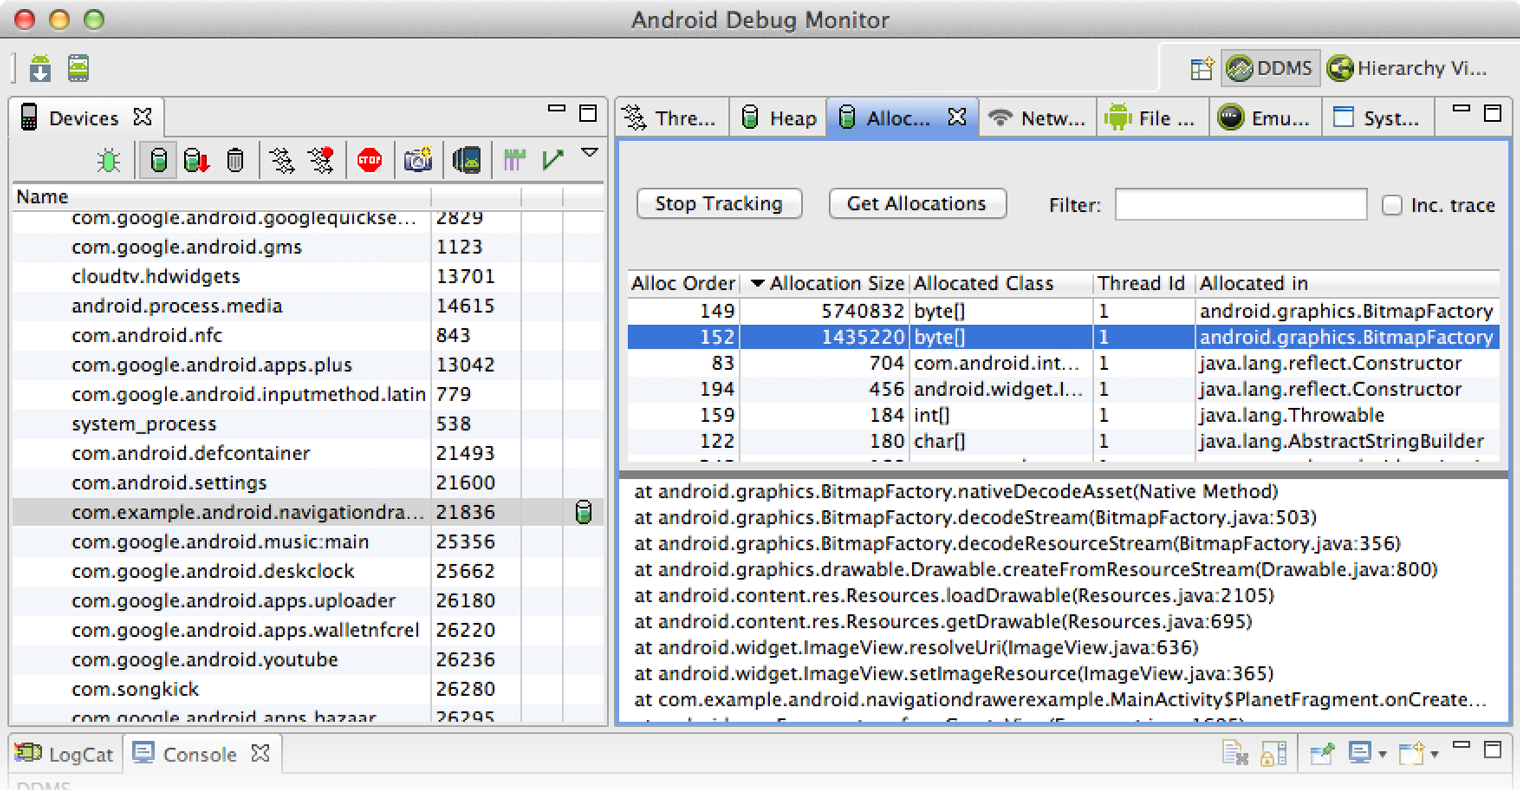
\includegraphics[width=140mm]{img/android-debug-monitor.png}
\caption{Android debug monitor.}
\label{overflow}
\end{figure}

Za detaljniju analizu može se pogledati kako je memorija naše aplikacije podijeljena po raznim tipovima alokacije radnog spremnika pomoću \textit{adb} naredbe:

\begin{center}
\verb=adb shell dumpsys meminfo <package_name | pid> [-d]=
\end{center}
koja će dati rezultat sličan ovome:

\begin{figure}[ht!]
\centering
\begingroup
    \fontsize{9pt}{12pt}\selectfont
		\begin{verbatim}
		** MEMINFO in pid 18227 [com.google.android.apps.maps] **
		                   Pss  Private  Private  Swapped     Heap     Heap     Heap
		                 Total    Dirty    Clean    Dirty     Size    Alloc     Free
		                ------   ------   ------   ------   ------   ------   ------
		  Native Heap    10468    10408        0        0    20480    14462     6017
		  Dalvik Heap    34340    33816        0        0    62436    53883     8553
		  ...
		  ...
		        TOTAL   216524   208232     4384        0    82916    68345    14570
\end{verbatim}
\endgroup
%\includegraphics[width=120mm]{img/example.png}
\caption{Analiza memorije procesa.}
\label{overflow}
\end{figure}

\noindent
i ovdje nam je bitno raspoznati dvije stvari:


\paragraph{•}
\textbf{Privatni čisti i prljavi radni spremnik} \textit{(engl. Private Clean and Dirty RAM)}\\
Ovo je količina memorije koju koristi naš proces i to je onaj dio memorije koji sustav može dobiti nazad nakon uništavanja istog. Ovdje je najbitnije gledati prljavi dio radnog spremnika, koji je ujedno i najskuplji, jer se tim djelom koristi samo naš process i ne može se straničiti na disk.

\paragraph{•}
\textbf{Proporcionalna veličina skupa} \textit{(engl. Proportional Set Size, PSS)}\\
Ovo je količina memorije koju koristi naša aplikacija uzimajući u obzir dijeljenje stranica kroz više procesa. Svaka stranica koja je jedinstvena za naš process direktno pridonosi ovoj vrijednosti, dok ostale stranice koje se dijele s drugim procesima doprinose proporcionalnu vrijednost dijela kojeg zauzimaju.

\subsection{Korištenje više procesa}
\paragraph{}
Iako velika većina aplikacija ne bi smjela koristiti više procesa u isto vrijeme, jer bi se mogli opeći i umjesto smanjenja, povećati iznos otiska \textit{(engl. footprint)} aplikacije u radnoj memoriji. No ako se ipak ide ovim putem mora se obratiti pažnja kakve će to utjecaje imati na našu memoriju.\\

Za ilustraciju posljedica zamislit će se jedan prazni process koji ne radi apsolutno ništa, i takav process ima dodatnih 1.4MB otiska u radnoj memoriji.

\begin{figure}[ht!]
\centering
\begingroup
    \fontsize{8pt}{12pt}\selectfont
		\begin{verbatim}
adb shell dumpsys meminfo com.example.android.apis:empty

** MEMINFO in pid 10172 [com.example.android.apis:empty] **
                Pss     Pss  Shared Private  Shared Private    Heap    Heap    Heap
              Total   Clean   Dirty   Dirty   Clean   Clean    Size   Alloc    Free
             ------  ------  ------  ------  ------  ------  ------  ------  ------
  Native Heap     0       0       0       0       0       0    1864    1800      63
  Dalvik Heap   764       0    5228     316       0       0    5584    5499      85
 Dalvik Other   619       0    3784     448       0       0
        Stack    28       0       8      28       0       0
    Other dev     4       0      12       0       0       4
     .so mmap   287       0    2840     212     972       0
    .apk mmap    54       0       0       0     136       0
    .dex mmap   250     148       0       0    3704     148
   Other mmap     8       0       8       8      20       0
      Unknown   403       0     600     380       0       0
        TOTAL  2417     148   12480    1392    4832     152    7448    7299     148
		\end{verbatim}
\endgroup
%\includegraphics[width=120mm]{img/example.png}
\caption{Analiza memorije praznog procesa.}
\label{overflow}
\end{figure}

Može se primijetiti da veličina nije baš zanemariva, i isto tako brzo i raste porastom kompleksnosti posla tog procesa. Na primjer, process koji prikazuje jedan \textit{Activity} sa tekstom će zauzeti 4MB, što je tri puta više, i to samo za prikazivanje običnog teksta na UI.\\

Ovime dolazimo do konkretnog zaključka, ako već moramo podijeliti aplikaciju u procese, isključovo jedan process mora biti zadužen za UI, a ostali moraju izbjegavati bilo kakvo korištenje UI elemenata, jer u suprotnom ćemo napuniti memoriju u kratkom roku.\\

Dodatno pošto se aplikacija vrti u više procesa mora se puno više fokusa uložiti u optimizaciju korištenja memorije u kodu jer se u ovom slučaju svaki propust replicira na druge procese i stvara sve veći problem.

\pagebreak
\chapter{Procesi i dretve}
\section{Uvod}
\paragraph{}
Pri pokretanju nove aplikacije, ako aplikacija nema niti jednu komponentu već pokrenutu, Android će pokrenuti novi Linux proces za tu aplikaciju s jednom dretvom. Po pravilu, sve komponente iste aplikacije pokreću se u istom procesu i dretvi -glavna dretva \textit{(engl. main thread)}. Ako prilikom pokretanja neke komponente već postoji proces koji je zadužen za tu aplikaciju (jer postoji neka druga komponenta koja je već pokrenuta) onda se nova komponenta pokreće unutar toga procesa i koristi istu dretvu za izvršavanje. Naravno, ako želimo, možemo svaku komponentu specifično izdvojiti u drugi proces ili napraviti više dretvi za bilo koji proces.

\section{Procesi}
\paragraph{}
Iako su sve komponente po pravilu pokrenute u istom procesu (i to se u većini slučajeva ne bi trebalo mijenjati), mi imamo potpunu kontrolu nad njima i može se lako promijeniti proces kojem će komponenta pripadati. To se radi u \textit{AndroidManifest.xml} datoteci. Svaki unos elementa android komponente u \textit{manifestu} - \verb|<activity>,| \verb|<service>, <receiver>, <provider>| - sadrži atribut \textit{android:process} gdje možemo specificirati ime procesa u kojem će komponenta živjeti.

\begin{figure}[ht!]
\centering
\begingroup
    \fontsize{10pt}{12pt}\selectfont
		\begin{lstlisting}
        <activity android:icon="drawable resource"
            android:label="string resource"
            android:name="string"
          	    . . .
            android:process="string"
          	    . . .
        </activity>
		\end{lstlisting}
\endgroup
%\includegraphics[width=120mm]{img/example.png}
\caption{\textit{Activity} element unutar AndroidManifest.xml.}
\label{overflow}
\end{figure}

Isto tako, \verb|| element podržava \textit{android:process} atribut koji onda postavlja unaprijed zadanu \textit{(engl. default)} vrijednost za sve komponente aplikacije. Unaprijed zadano ime procesa odgovara imenu paketa aplikacije koje je određeno u \textit{manifestu}.\\

Ako ime procesa počinje s dvotočkom \textit{(':')}, novi privatan proces za aplikaciju stvara se tek onda kada je potreban i komponenta se pokrene unutar njega. U slučaju da ime procesa započinje malim slovom, \textit{activity} će se pokrenuti u globalnom procesu tog imena ako ima ovlasti za to. Ovime se omogućuje komponentama iz različitih aplikacija da dijele procese, te smanjujemo potrošnju resursa.\\

Android se u bilo kojem trenutku može odlučiti ubiti proces, kad je memorija pri kraju, a drugi procesi koji su trenutačno važniji za posluživanje korisnika ju zahtijevaju. U tom slučaju komponenta aplikacije bude uništena skupa s procesom, i oni se ponovno pokreću kada se to od njih bude tražilo.


\subsection{Život procesa}
\paragraph{}
Android ima u cilju što duže zadržati proces aplikacije živim, dok ga eventualno ne uništi kako bi oslobodio memoriju za nove ili važnije procese. Za takvu vrstu odluke procesi se stavljaju u hijerarhiju po važnosti. Ta hijerarhija bazirana je na pokrenutim komponentama u procesu i njihovom trenutnom stanju, te se onda postepeno izbacuju procesi od najmanje važnosti.\\

Postoji pet stupnjeva \textit{hijerarhije po važnosti}. U sljedećoj listi prikazani su različiti tipovi procesa po važnosti (prvi je najvažniji, odnosno zadnji se ubija):

\begin{enumerate}
\item
\textbf{Proces u prvom planu} \textit{(engl. Foreground process)}\\
Proces koji je potreban za ono što korisnik trenutno radi i vidi. Smatra se da je proces u prvom planu ako je ispunjen jedan od slučajeva:
	\begin{itemize}
	\item sadrži \textit{activity} s kojim korisnik komunicira – pozvana \textit{onResume()} metoda nad \textit{activity-em}
	\item sadrži servis koji je povezan s \textit{activity-em} s kojim korisnik komunicira
	\item sadrži servis koji je pokrenut u prvom planu – pozvana \textit{startForeground()} metoda servisa
	\item sadrži servis koji pokreće jedan od svojih glavnih ugrađenih poziva – \textit{onCreate(), onStart() ili onDestroy()}
	\item sadrži \textit{BroadcastReceiver} koji trenutno izvršava \textit{onReceive()} metodu
	\end{itemize}
Realno će  u bilo kojem danom trenutku biti svega par takvih procesa upaljenih i njihovo se ubijanje smatra zadnjom opcijom, a to je kada nema dovoljno memorije da se svi izvršavaju odjednom. U tom trenutku uređaj je u stanju straničenja memorije, pa je ubijanje ovih procesa potrebno kako bi održali UI responzivnim.	
	
\item
\textbf{Vidljivi procesi}\\
Proces je vidljiv ako nema nijednu komponentu u prvom planu, ali utječe na ono što korisnik vidi na ekranu. Smatra se da je proces vidljiv ako je ispunjen jedan od slučajeva:
	\begin{itemize}
	\item sadrži \textit{activity} koji nije u prvom planu, ali je vidljiv korisniku – pozvana \textit{onPause()} metoda (npr. kad se otvori dijalog, roditeljski \textit{activity} je još uvijek vidljiv ispod njega)
	\item sadrži servis koji je vezan za vidljivi ili \textit{activity} u prvom planu
	\end{itemize}
Ovakav se proces smatra iznimno važnim i neće se dirati ako to nije potrebno da bi procesi u prvom planu preživjeli.

\item
\textbf{Proces Servisa}\\
Proces koji ima pokrenut servis sa \textit{startService()} metodom i koji nije pripadnik prve dvije kategorije.\\
Iako servisi inače nisu direktno povezani s onime što korisnik vidi, oni rade stvari koje su bitne za krajnjeg korisnika (npr. puštanje muzike u pozadini) tako da ih Android drži živima dok ima dovoljno memorije da prežive i procesi u prvom planu i svi vidljivi procesi.

\item
\textbf{Proces u pozadini}\\
Proces koji sadrži \textit{activity} koji trenutno nije vidljiv korisniku – pozvana je\linebreak \textit{onStop()} metoda.\\
Takvi procesi nemaju nikakav utjecaj na UX, tako da ih Android u bilo kojem trenutku može ubiti s ciljem oslobađanja memorije. Realno u bilo kojem danom trenutku biti će puno procesa koji se izvode u pozadini, i oni se spremaju u LRU priručnu memoriju kako bi se osiguralo pravedno uništavanje aplikacija po prioritetu najmanjeg korištenja istih.

\pagebreak
\item
\textbf{Prazan proces}\\
Proces koji ne sadrži niti jednu aktivnu komponentu aplikacije.\\
Jedini razlog da bi uopće postojao ovakav proces je zbog korištenja priručne memorije i bržeg pokretanja komponenti koje će se unutar ovog procesa pokretati u budućnosti.

\end{enumerate}

Tijekom rangiranja procesa Android će uzeti najveći mogući stupanj hijerarhije koji je zadovoljen. Ako proces sadrži i servis i vidljivi \textit{activity}, biti će rangiran kao vidljivi proces, a ne kao proces servisa.\\

Isto tako, proces može biti promaknut ako postoji neki drugi proces koji ovisi o njemu – jer proces ne smije biti manje rangiran od procesa kojeg poslužuje. Dobar primjer za to daju \textit{ContentProvider} klase ili servisi koji su vezani za neku komponentu u drugom procesu.\\

Može se primijetiti da je proces servisa više rangiran od procesa u pozadini, tako da ako u aplikaciji radimo neki posao koji ima veće trajanje nego obično (npr. upload datoteke) najbolje je da sav posao prebacimo u novi servis nego da ga odrađujemo na radnoj dretvi \textit{(engl. worker thread)}. Time dobivamo sigurnost da će proces biti rangiran kao proces servisa, bez obzira na to što se dogodi sa \textit{activity-em}. Iz istog razloga je i dobra praksa u \textit{BroadcastReceiver} klasi uposliti servise umjesto da opterećujemo dretvu.

\subsection{Komunikacija između procesa}
\paragraph{}
Za komunikaciju između različitih procesa Android koristi RPC pozive \textit{(engl. Remote Procedure Call, RPC)}, gdje poziva metodu iz \textit{activityj-a} ili neke druge komponente aplikacije i ista se izvršava u drugom procesu, te nakon izvršavanja vraća rezultat pozivatelju. Na ovaj se način poziv metode rastavlja na nivo operacijskog sustava i prenosi se iz lokalnog procesa i adresnog prostora na drugi proces i njegov adresni prostor te tamo izvršava naredbe pozvane metode i vraća rezultat na isti način u drugom smjeru. Android rješava sav kod za transakcije komunikacije između procesa \textit{(engl. Interprocess Communication, IPC)} tako da je sve što se treba napraviti definicija i implementacija RPC sučelja (engl. interface).\\

Kako bi obavili IPC komunikaciju, aplikacija se mora vezati za servis metodom \textit{bindService()} koja vraća klijent-server sučelje preko kojeg komponente aplikacije komuniciraju sa servisom. Takav povezani servis \textit{(engl. Bound Service)} živi sve dok ima neku komponentu bilo koje druge aplikacije povezanu na sebe. Pošto je moguće spojiti više komponenata odjednom na jedan takav servis, u trenutku kada se sve komponente odspoje, servis će se uništiti. Na ovaj način otvaramo dostupnost djela funkcionalnosti naše aplikacije ostalim aplikacijama preko IPC komunikacije.\\

Da bi kreirali vezani servis, mora se implementirati \textit{onBind()} metoda ugrađenog poziva gdje se vraća \textit{IBinder} koji služi kao sučelje za komunikaciju sa samim servisom. Nakon toga ostale se komponente mogu jednostavno spojiti na servis pozivajući \textit{bindService()} metode nakon čega dobivaju sučelje preko kojega mogu početi pozive metoda na servisu. Kako se operacijski sustav brine za uništavanje vezanih servisa kada ne postoji niti jedna komponenta vezana za njega, znači da nije potrebno ručno zaustavljanje ovakvog servisa.
 
\section{Dretve}
\paragraph{}
Pri pokretanju aplikacije, sustav kreira glavnu dretvu odgovornu za izvršavanje\linebreak programa pod nazivom "glavna dretva" \textit{(engl. main thread)}. Ova dretva je praktički najvažnija u cijeloj aplikaciji jer delegira slanje svih događaja \textit{(engl. event)} na odgovarajuće elemente grafičkog sučelja \textit{(engl. User Interface, UI)}, uključujući i događaje vezane za crtanje. Također u toj se dretvi odvija interakcija s ostalim komponentama iz \textit{Android UI toolkit} paketa, te kao takva, glavna se dretva ponekad naziva i "UI" dretva.\\

Sve komponente aplikacije koje se vrte u istom procesu pokreću se na UI dretvi i sustav nikada ne kreira nove dretve za svaku instancu komponente. Isto tako i sistemski pozivi aplikacije, kao i metode za odgovor na sistemski ugrađeni poziv uvijek se pokreću na UI dretvi procesa. Na primjer, kada korisnik pritisne gumb na ekranu, aplikacija šalje događaj dodira elementu, nakon čega se isti postavi u kliknuto stanje, te invalidira događaj u redu događaja \textit{(engl. event queue)}. Nakon toga UI dretva miče događaj iz reda i obavještava element da se promijenio i da se mora ponovno nacrtati.\\

Ovakav jednodretveni model ima i jednu jako veliku manu. U slučaju da aplikacija obrađuje jako veliku količinu posla kao rezultat neke akcije od strane korisnika, to može rezultirati jako lošim performansama aplikacije ako se to napravi na krivi način. Kada bi se sav taj posao odrađivao na UI dretvi, ona bi automatski postala blokirana dok se posao ne obavi do kraja, što bi značilo nemogućnost slanja nikakvih daljnjih događaja, uključujući i one za crtanje. Gledajući iz perspektive korisnika, aplikacija će se smrznut i prestati reagirati, a ukoliko bude smrznuta više od 5 sekundi, Android će pokazati korisniku poznati \textit{"application not responding" (ANR)} dijalog. Korisnik se tada može odlučiti na ubijanje aplikacije i pobrisati ju s uređaja ako je nezadovoljan istom. Ovakva situacija bi se svakako trebala izbjeći pod svaku cijenu.\\

Još jedan jako bitan detalj je da \textit{Android UI toolkit} nije dretveno osiguran \textit{(engl. thread-safe)}, što bi značilo da se njegovi elementi ne mogu mijenjati iz više dretvi istovremeno. Iz tog se razloga ne smije manipulirati UI elementima iz druge dretve, već se sva manipulacija na UI elementima radi na UI dretvi.\\

Iz ovog osnovnog pogleda na dretve u Androidu okruženju izašla su dva zlatna pravila za ovakav jednodretveni model kojih bi se svatko trebao držati:

\begin{enumerate}
\item Nikada ne blokirati UI dretvu
\item Nikada ne pristupati \textit{Android UI toolkit} elementima od izvana UI dretve
\end{enumerate}

\subsection{Radna dretva}
\paragraph{}
Poštujući prvo pravilo jako je bitno ne blokirati UI dretvu zbog responzivnosti cijele aplikacije. Ukoliko dođe situacija da neki posao nije moguće odmah izvršiti, već je potrebno neko vrijeme za to (npr. dohvaćanje slike sa interneta), takvu stvar moramo staviti u posebnu dretvu - "pozadinska" \textit{(engl. background thread)}  ili "radna" dretva \textit{(engl. worker thread)}.\newpage
Ovo je primjer kako u slušatelju za događaj klika \textit{(engl. click listener)} dohvaćamo sliku s interneta na radnoj dretvi i prikazujemo ju u \textit{ImageView}:

\begin{figure}[ht!]
%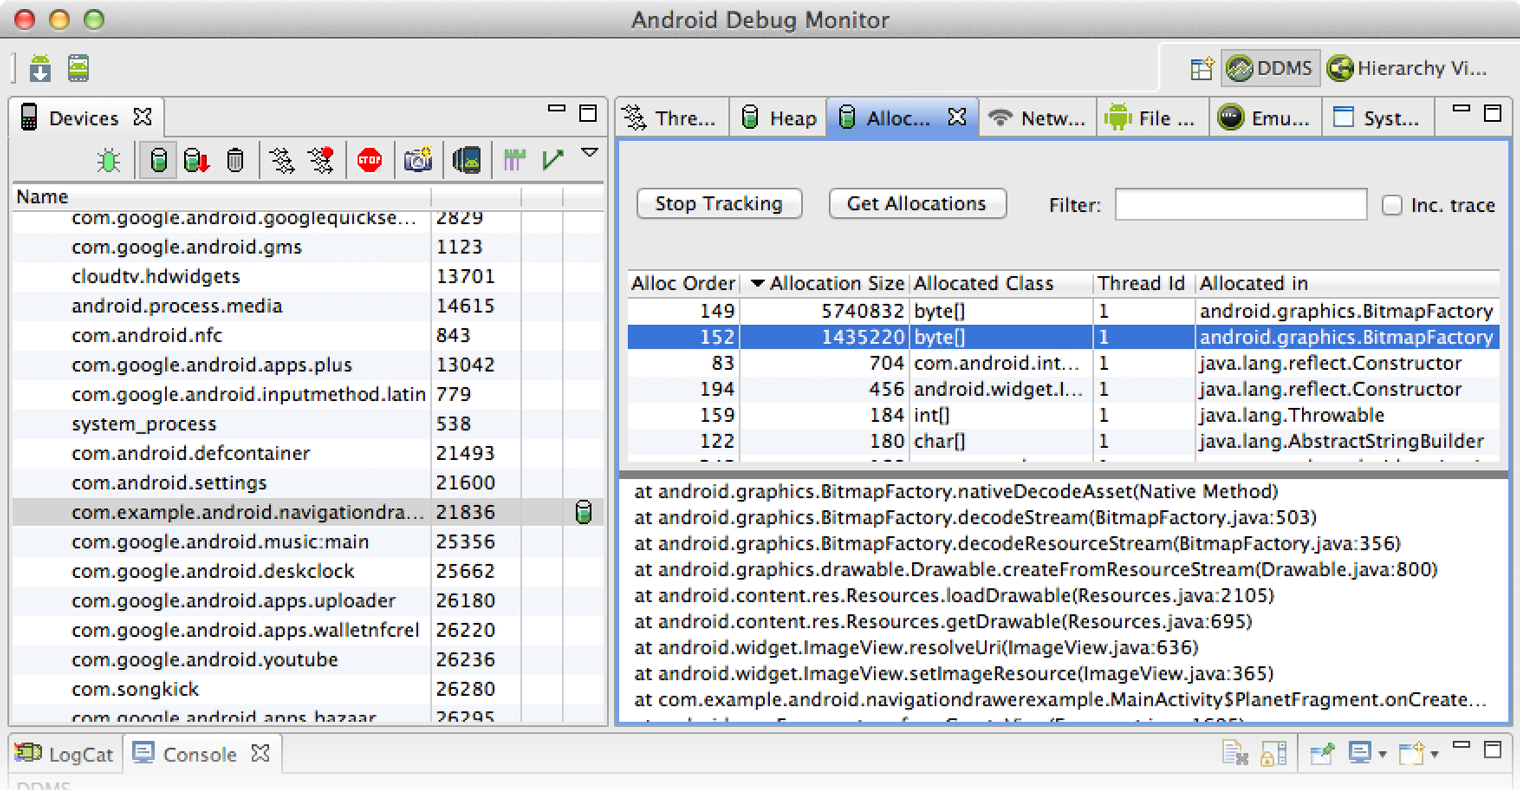
\includegraphics[width=140mm]{img/android-debug-monitor.png}
\begin{lstlisting}
public void onClick(View v) {
    new Thread(new Runnable() {
        public void run() {
            Bitmap bitmap = loadImageFromNetwork("http://example.com/image.png");
            mImageView.setImageBitmap(bitmap);
        }
    }).start();
}
\end{lstlisting}
\caption{Dohvaćanje slike u radnoj dretvi.}
\label{overflow}
\end{figure}

Na prvi pogled sve se čini ok, napravila se nova dretva koja onda dohvaća sliku i stavi je u \textit{imageView} kako je i planirano. Međutim, kada se sjetimo drugog pravila dretvi koje govori da se nikako ne smije pristupati \textit{Android UI toolkit} elementima izvan UI dretve, uviđamo da se upravo to događa u ovoj novoj radnoj dretvi. Ovaj kod može rezultirati neočekivanim ponašanjem aplikacije i samim time se produljuje i otežava razvoj aplikacije i lovljenje bugova.\\

Ovo je poznati problem i Android nudi nekoliko rješenja:
\paragraph{•}
\textit{Activity.runOnUiThread(Runnable action)}
\paragraph{•}
\textit{View.post(Runnable action)}
\paragraph{•}
\textit{View.postDelay(Runnable action, long delay)
}\\

Metode primaju \textit{Runnable} akciju koja će se izvršiti na UI dretvi i isto tako se može dodati parametar \textit{delay} tipa \textit{long} koji predstavlja milisekunde čekanja prije nego se akcija izvrši na UI dretvi.\newpage 
Navedeni primjer može odmah popraviti:

\begin{figure}[ht!]
%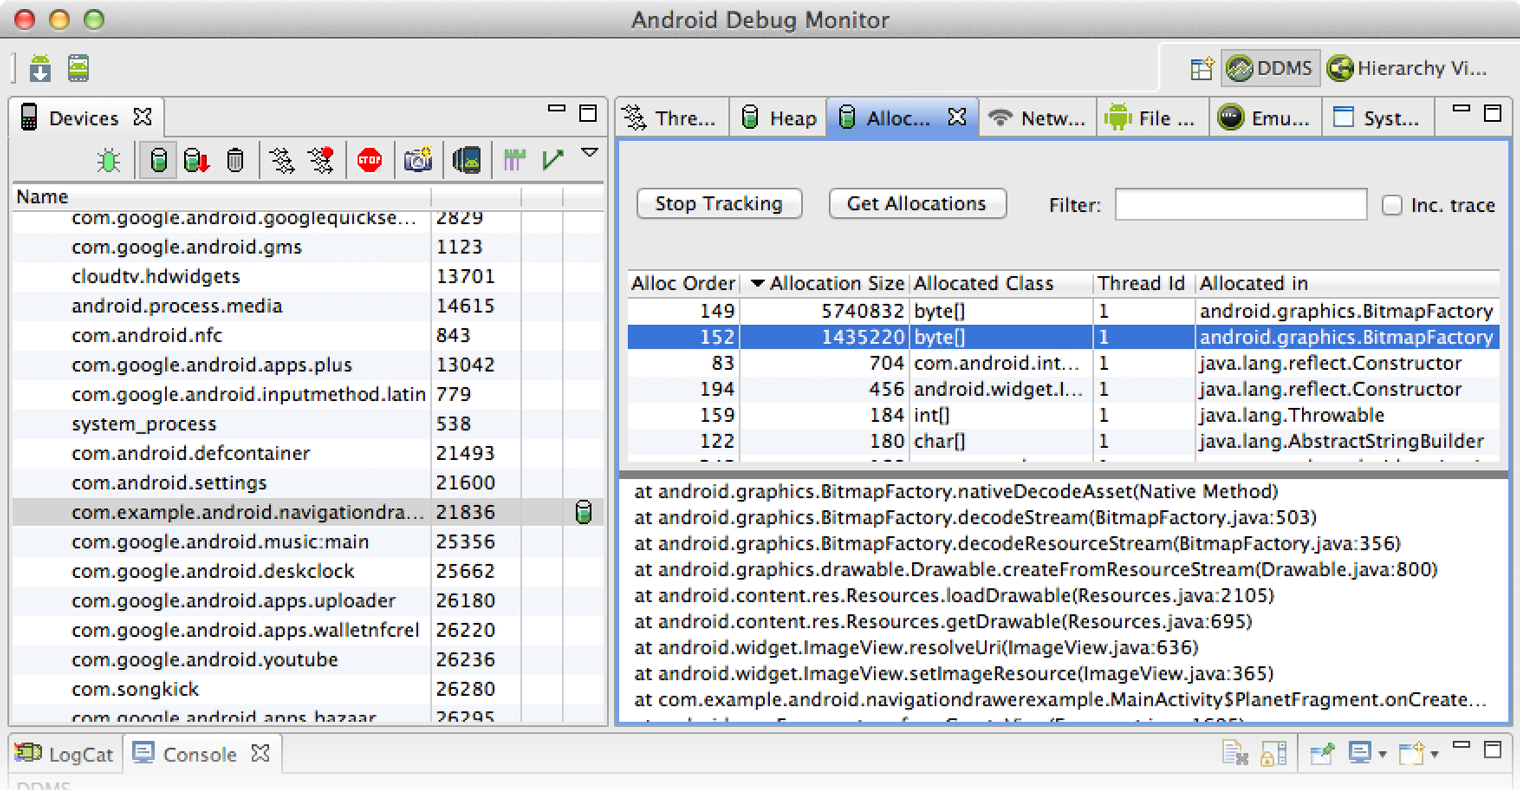
\includegraphics[width=140mm]{img/android-debug-monitor.png}
\begin{lstlisting}
public void onClick(View v) {
    new Thread(new Runnable() {
        public void run() {
            final Bitmap bitmap =
                    loadImageFromNetwork("http://example.com/image.png");
            mImageView.post(new Runnable() {
                public void run() {
                    mImageView.setImageBitmap(bitmap);
                }
            });
        }
    }).start();
}
\end{lstlisting}
\caption{Osvježavanje slike na UI dretvi.}
\label{overflow}
\end{figure}

Može se primijetiti da je ovaj kod u potpunosti dretveno osiguran, dohvaćanje slike obavlja se u zasebnoj dretvi, dok se manipulacija \textit{ImageView-a} odvija na UI dretvi.\\

Isto tako može se vidjeti da kako se povećava kompleksnost operacija, ovakvo rješenje postaje sve kompliciranije i teže za održavanje. Ovdje će pomoći korištenje rukovatelja \textit{(engl. Handler)} u radnoj dretvi koji procesuira poruke dobivene sa UI dretve, a još bolje rješenje bi bilo proširivanje \textit{(engl. extend)} \textit{AsyncTask} klase jer pojednostavljuje pisanje koda koji bi se odvijao na radnoj dretvi i komunicirao sa UI elementima na UI dretvi.

\subsection{klasa \textit{AsyncTask}}
\paragraph{}
Klasa \textit{AsyncTask} omogućuje i olakšava pravilno korištenje UI dretve. Ona služi za izvršavanje blokirajućih operacija u pozadini i prikazivanje rezultata na UI dretvi bez potrebe da sami manipuliramo dretvama i rukovateljima. Stoga je \textit{AsyncTask} zapravo pomoćna klasa vezana za \textit{Thread} i \textit{Handler} i nije zamišljen kao radno okruženje za baratanje dretvama. Idealno se koristi za operacije do svega par sekundi, a za sve ostale stvari koje bi se trebale duže vrtit u pozadini koriste se API koji se nalaze u java.util.concurrent paketu (npr. Executor, ThreadPoolExecutor, FutureTask).\\

Svaki AsyncTask definiran je sa tri generička tipa Params, Progress i Result, i možemo ga podijeliti u 4 koraka izvršavanja onPreExecute, doInBackground, onProgressUpdate i onPostExecute.\\

Da bi ga koristili svakako ga moramo napraviti odgovarajuću subklasu gdje ćemo implementirati doInBackground() metodu koja se zatim pokreće u pool-u dretvi u pozadini. Osvježavanje UI elemenata radimo u onPostExecute() metodi gdje dobivamo rezultat iz doInBackground() dijela i pokreće promjene na UI dretvi. Kad smo gotovi task se pokreće metodom execute().


\chapter{Zaključak}
Zaključak.

\bibliography{literatura}
\bibliographystyle{fer}

\begin{sazetak}
Sažetak na hrvatskom jeziku.

\kljucnerijeci{Ključne riječi, odvojene zarezima.}
\end{sazetak}

% TODO: Navedite naslov na engleskom jeziku.
\engtitle{Title}
\begin{abstract}
Abstract.

\keywords{Keywords.}
\end{abstract}

\end{document}
